% $Id: template.tex 11 2007-04-03 22:25:53Z jpeltier $

%\documentclass{vgtc}                          % final (conference style)
\documentclass[review]{vgtc}                 % review
%\documentclass[widereview]{vgtc}             % wide-spaced review
%\documentclass[preprint]{vgtc}               % preprint
%\documentclass[electronic]{vgtc}             % electronic version

%% Uncomment one of the lines above depending on where your paper is
%% in the conference process. ``review'' and ``widereview'' are for review
%% submission, ``preprint'' is for pre-publication, and the final version
%% doesn't use a specific qualifier. Further, ``electronic'' includes
%% hyperreferences for more convenient online viewing.


\usepackage{mathptmx}
\usepackage{graphicx}
\usepackage{times}

\onlineid{0}

%% declare the category of your paper, only shown in review mode
\vgtccategory{Research}

%% allow for this line if you want the electronic option to work properly
\vgtcinsertpkg

%% In preprint mode you may define your own headline.
%\preprinttext{To appear in an IEEE VGTC sponsored conference.}

%% Paper title.

\title{Hierarchical qualitative color palettes}

\author{Martijn Tennekes\thanks{e-mail: m.tennekes@cbs.nl}\\ %
        \scriptsize Statistics Netherlands %
\and Edwin de Jonge\thanks{e-mail:e.dejonge@cbs.nl}\\ %
     \scriptsize Statistics Netherlands}

\abstract{ Color is an important means to display categorical data in statistical graphics. Categories are often hierarchically structured in a classification tree, but most qualitative color palettes do not take this hierarchy into account.  

We present a method to map tree structures to colors from the Hue-Chroma-Luminance (HCL) color model. The HCL color space, which is a transformation of the CIELUV color space, is known for its well balanced perceptual properties. Our experiments suggest that hierarchical qualitative color palettes are very useful: not only for improving standard hierarchical visualizations such as trees and tree maps, but also for showing tree structure in non-hierarchical visualizations.
}

\CCScatlist{ 
 \CCScat{H.5.2}{ Information Interfaces and Presentation}%
{User Interfaces}{User-centered design}
}

%% Copyright space is enabled by default as required by guidelines.
%% It is disabled by the 'review' option or via the following command:
% \nocopyrightspace

\graphicspath{{../plots/}}

\begin{document}

\firstsection{Introduction}

\maketitle

Hierarchical data are of crucial importance in official statistics. Most official data are published using hierarchically structured categories, for instance geographic regions or economic activities. A recent trend in data analysis practice, is to follow a top-down approach rather than to check  each individual record of a survey or administrative source. Several data visualization methods are useful to explore and analyze hierarchical statistical data, for instance treemaps
\cite{shneiderman1992,tennekes2011b}. Color palettes reflecting the  hierarchical structure would be very useful in supporting visual analysis.

Assigning colors to categories is far from trivial. On the one hand, qualitative colors should be distinct, but on the other hand they should not suggest non-existent order or proximity and introduce perceptual bias. The selection of color palettes for categorical data first depends on the type of data. For nominal data, such as gender or nationality, qualitative color palettes are used, while for ordinal data, such as level of urbanization, sequential or diverging palettes are used \cite{brewer03, zeileis2009}. However, for hierarchical categories there are no specific guidelines for selecting color palettes, to the best of our knowledge.

Although many tree visualizations are proposed in literature \cite{schulz2011}, most of them use color to a small extent. A visualization technique that uses color as a major attribute is the InterRing \cite{yang2002}, a navigation tool with a radial layout. The leaf nodes are assigned to a different hue values. The color of a parent node is derived from averaging the colors of its children, where larger branches have more weight. An implicit effect is that colors of higher hierarchical levels are less saturated, except for one-child-per-parent branches.


\section{Method}


The Hue-Chroma-Luminance (HCL) space, which is a transformation of the CIELUV color space, is designed with the aim to control human color perception~\cite{ihaka2003}.
Colors with different hue values are perceptually uniform in colorfulness and brightness, which does not hold for the popular Hue-Saturation-Value (HSV) color space~\cite{zeileis2009}. We use the HCL space to select colors for hierarchical structures. The hue $H$ takes values from 0 to 360, and the chroma $C$ and luminance $L$ take values from 0 to 100.
We will use $H$ for the tree structure, where child nodes resemble the hue of their parent nodes. $C$ and $L$ will be used to show discrimate the different hierarchichal levels.

We illustrate our method with the European classification system of economic activity NACE \cite{nace}. Section F (Construction) is depicted in Figure~\ref{fig:sbiF}. The nodes are colored with the resulting hierarchical color palette. 

\begin{figure}[htb]
  \centering
  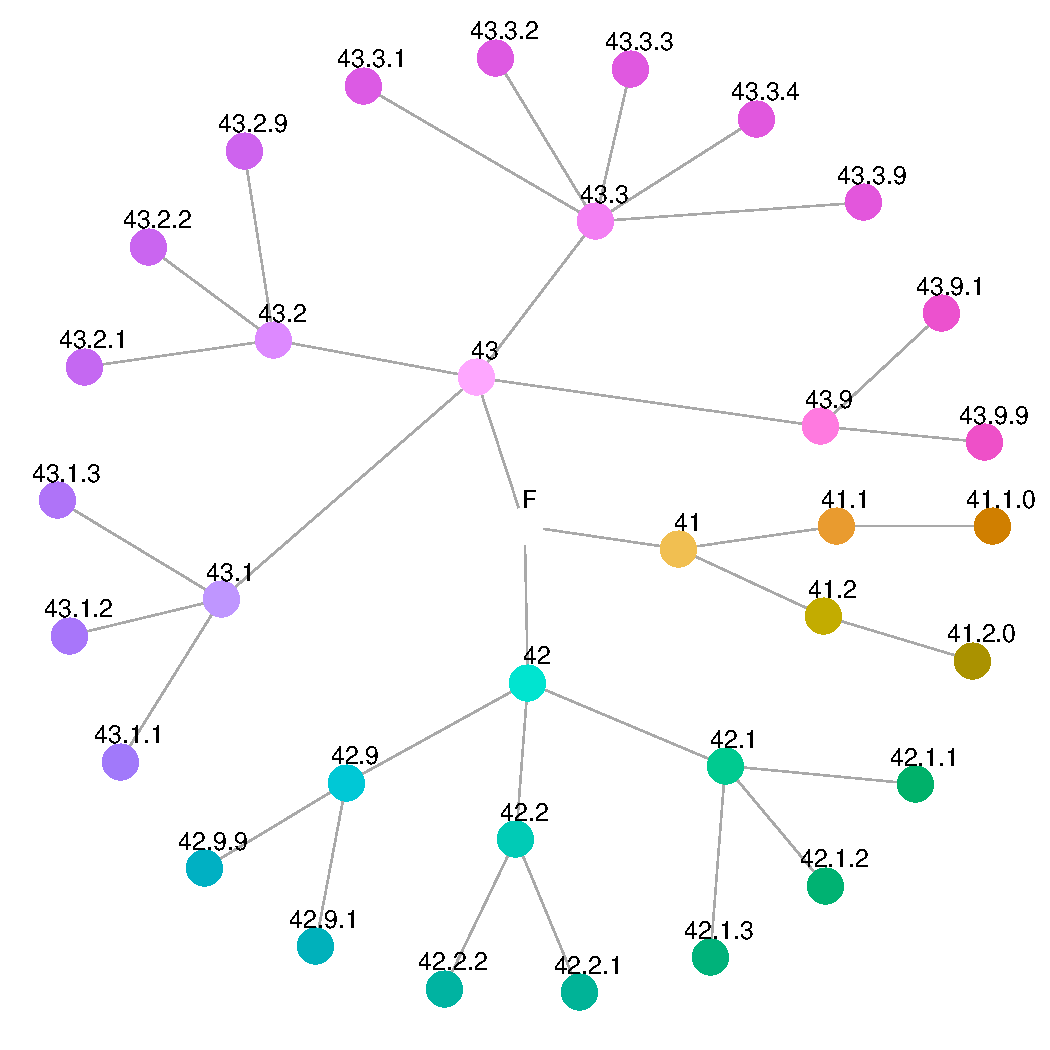
\includegraphics[width=3.5in]{sbi_F.pdf}
  \caption{Tree structure of economic sector F of NACE.}\label{fig:sbiF}
\end{figure}

For selecting hue values we use the following breadth-first algorithm. Starting with the root node, which is assigned to a predefined hue range (by default $[0, 360]$), the procedure per node $v$ is: 
\begin{enumerate} \itemsep1pt \parskip0pt 
\parsep0pt
\item assign the middle hue value in the hue range to $v$ (ignore coloring the root node itself);
\item if $v$ has children:
\begin{enumerate} \itemsep1pt \parskip0pt 
\parsep0pt
\item divide the hue range equally among $v$'s children;
\item keep the middle parts;
\item visit the $v$'s children.
\end{enumerate}
\end{enumerate}

\begin{figure}[htb]
  \centering
  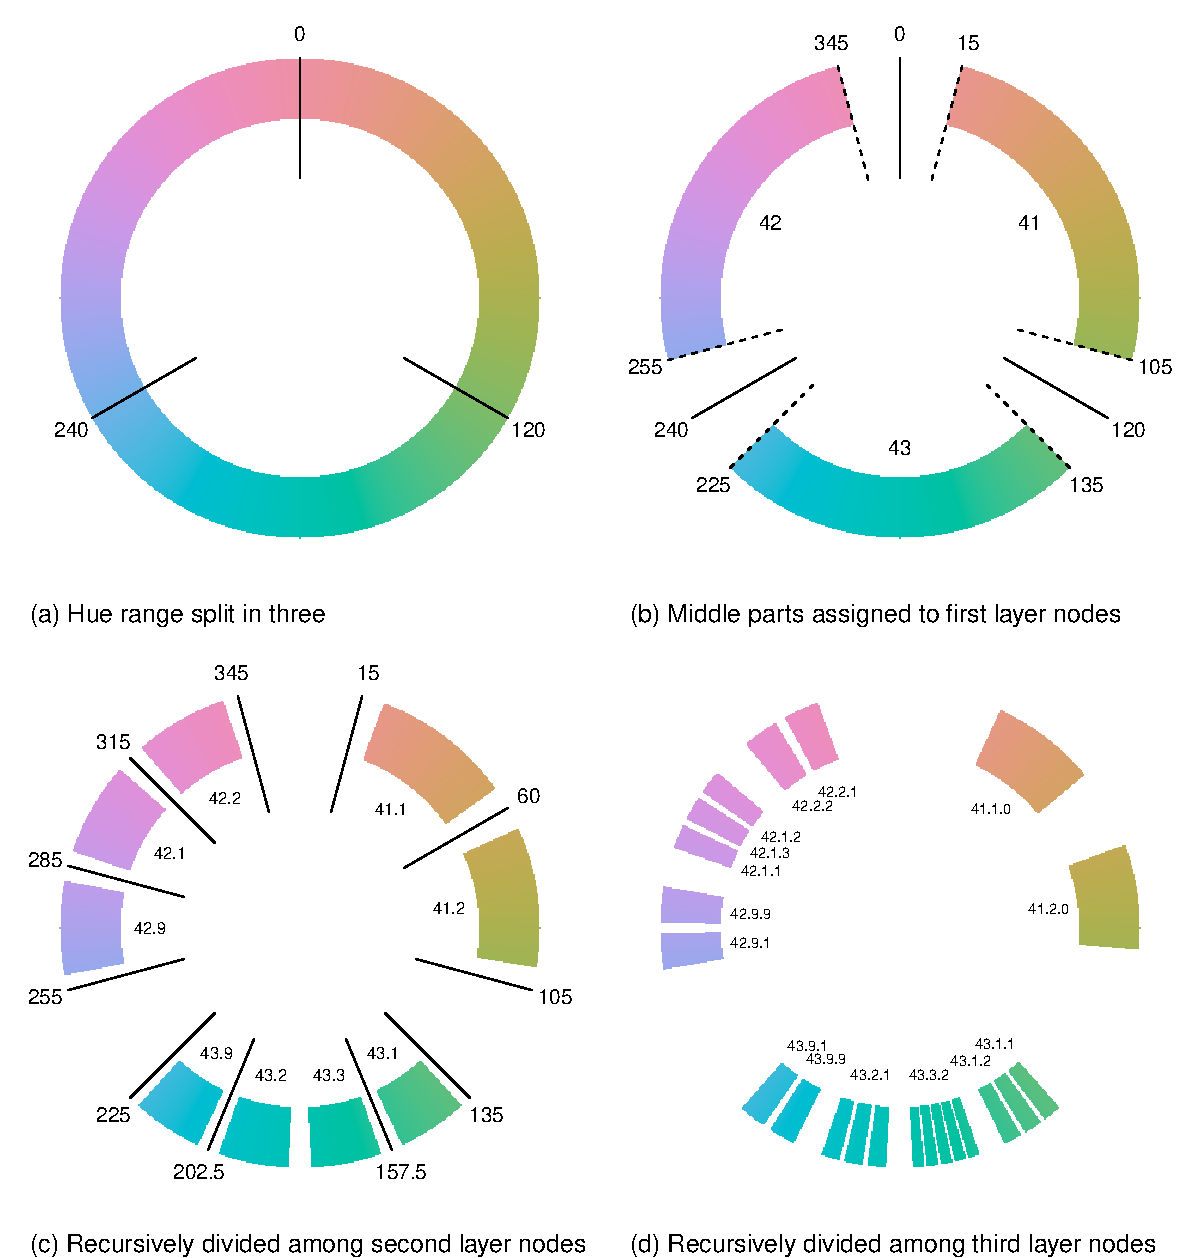
\includegraphics[width=3.5in]{hcl_method.pdf}
  \caption{Assignment of hue values.}\label{fig:wheel}
\end{figure}

This division of the hue range is illustrated in Figure~\ref{fig:wheel}: in (a) the full hue range (for a constant $C=60$ and $L=70$)  is divided among the three children of the root, in (b) the middle parts are kept, in (c) and (d) these steps are recursively taken for the deepest two hierarchical layers.

Ad 2(a) In most hierarchical structures, there is no ordinal order among siblings. When the nodes in such structure are plotted in a linear or radial layout, the colors of the siblings should not introduce a perceptual order. Therefore, the assigned hue ranges are permuted among the siblings. The used permutation order is based on the five-elements-permutation $[1, 3, 5, 2, 4]$. Furthermore, the permutation within even numbered branches is reversed to differentiate between branches. 

Ad 2(b) The fraction of each hue range that is kept is by default set to $0.75$. This choice is a trade-off between discriminating different main branches and discriminating different leaf nodes. 

In order to show depth, we let $C$ and $L$ values only depend on the depth of the corresponding nodes. We let the $L$ decrease linearly with depth and $C$ increase, analog to ocean water colors at various depths.

\begin{figure}[htb]
  \centering
  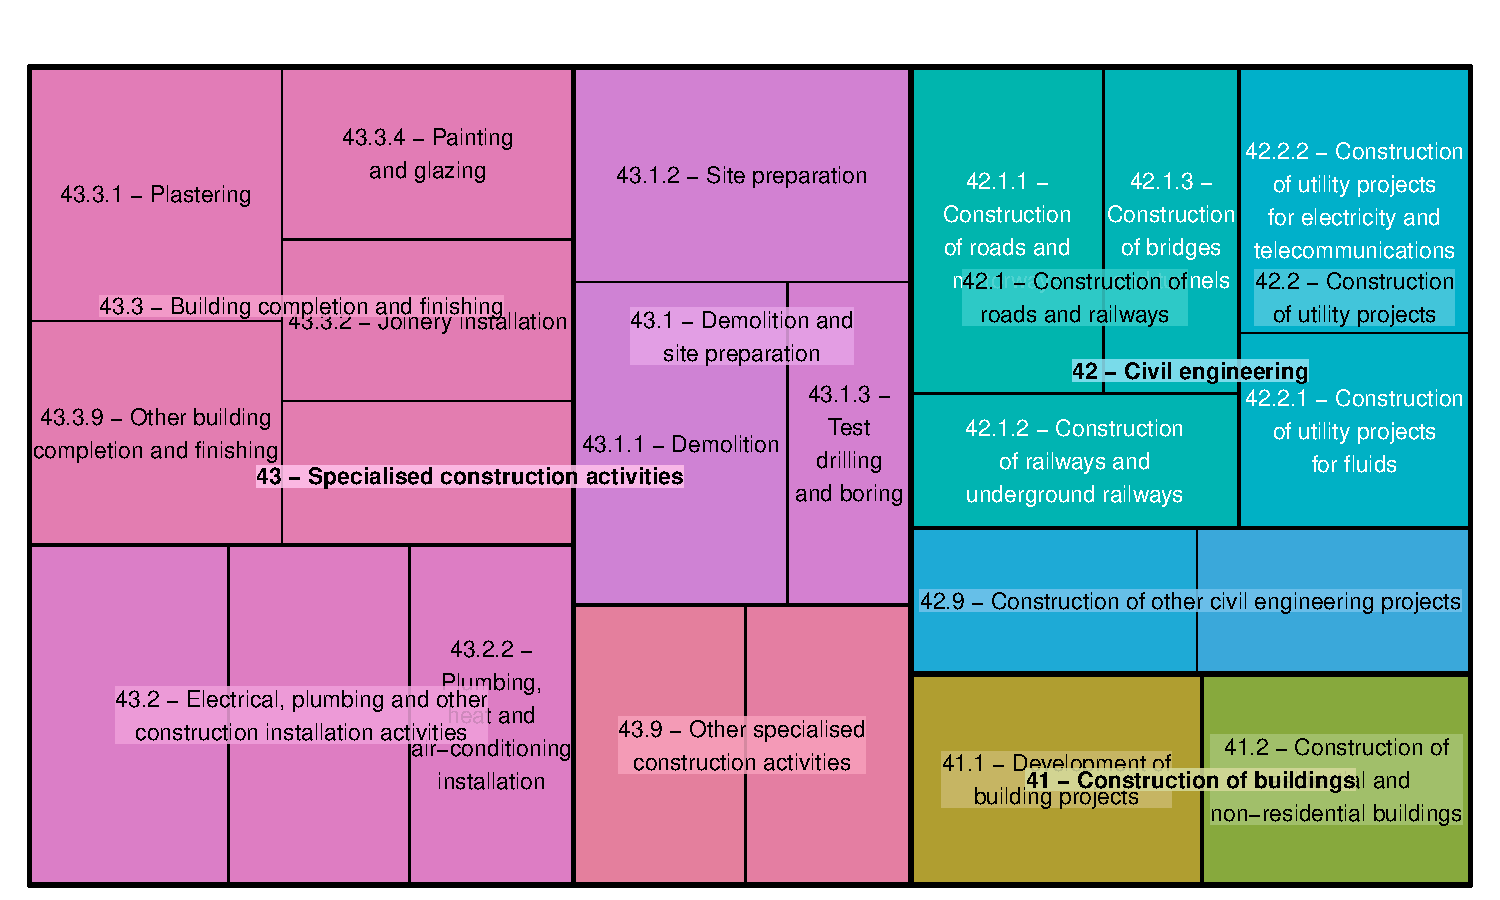
\includegraphics[width=3.5in]{treemap_F.pdf}
  \caption{Treemap with hierarchical colors}\label{fig:treemapF}
\end{figure}



\begin{figure}[htb]
  \centering
  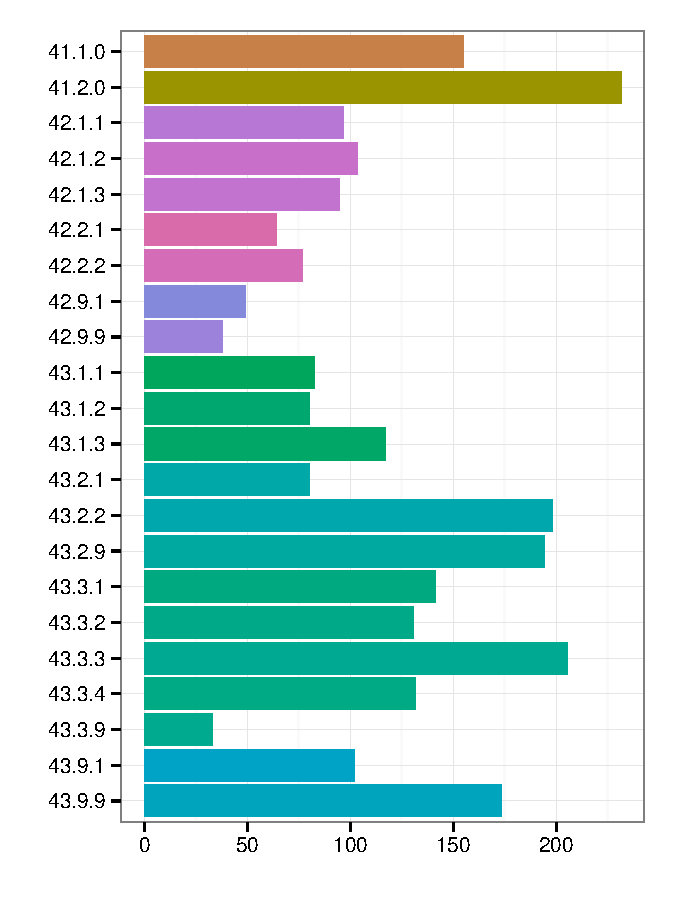
\includegraphics[width=1.75in]{bar_chart.pdf}
  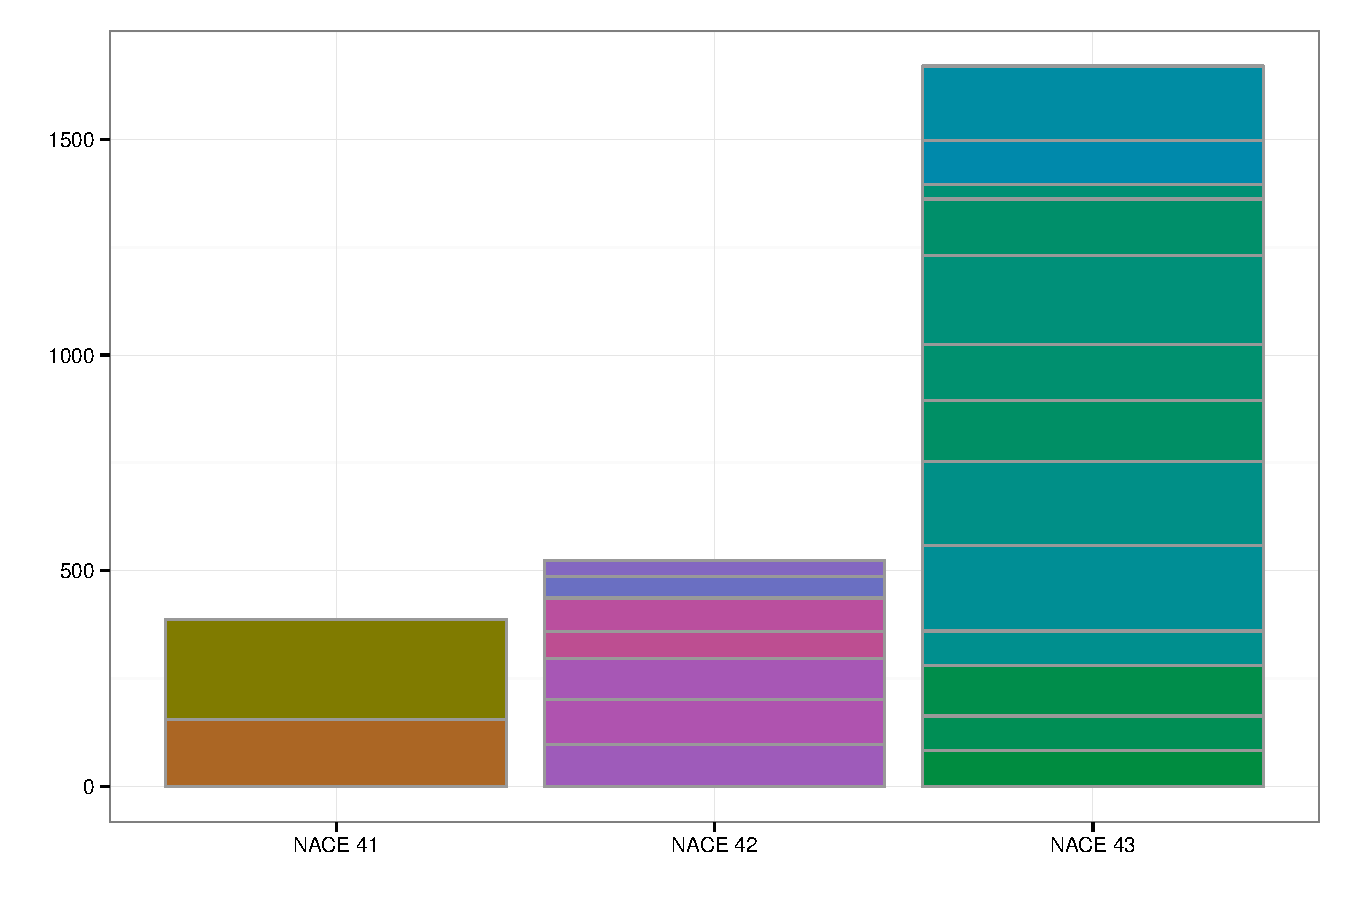
\includegraphics[width=1.75in]{stackedbar_chart.pdf}
  \caption{Bar chart with hierarchical colors}\label{fig:barchart}
\end{figure}



\section{Application}

A treemap of a random variable assigned to the NACE tree of sector F is depicted in Figure~\ref{fig:treemapF}. As a real application in official statistics, this variable could be turnover that is available for each business enterprise in a business register, and aggregated according to the NACE tree. The colored rectangles correspond to the deepest NACE layer, while the color of higher NACE layers is used to for the text label backgrounds. This treemap are created with the free and open source R package treemap \cite{treemap}.

As an example of a non-hierarchically-structured plot, a bar chart of random data is depicted in ~\ref{fig:barchart}. Such graphics could be useful when the hierarchical structure will not be the main focus in the conducted analyses. The stacked bar shows the internal structure .....

\section{Further research}

We recommend to further investigate the proposed hierarchical color selection method, and to evaluate the obtained color palettes in various statistical graphics.
[testen op eindgebruikers etc.]

%\acknowledgements{
%The authors wish to thank A, B, C. This work was supported in part by
%a grant from XYZ.}

\bibliographystyle{abbrv}
%%use following if all content of bibtex file should be shown
%\nocite{*}
\bibliography{hiercolor}
\end{document}
